\documentclass[12pt]{article}

\usepackage{preamble}



%title, author, date
\title{Netzwerkanalyse mit Wireshark: Welche (Meta-)daten werden weitergegeben?}
\author{Luis Herzog}
\date{April 2023}




\begin{document}





%Titlepage

\maketitle


\thispagestyle{empty}

\begin{figure}[h]
	\centering
	
\includegraphics[scale=0.1]{Bilder/Wireshark_icon.svg.png}
	\caption{Wireshark Logo}
	\label{fig:figure1}
\end{figure}


\newpage
\tableofcontents
\newpage

Es gibt viele verschiedenen Arten von Daten. Somit ebenfalls verschiedene Definitionen. 

Bevor man über die Wireshark Software sprechen kann, müssen die Basics geklärt werden:

\begin{itemize}
	\item Was sind Protokolle?
	\item Welche Protokolle gibt es?
	\item Wie funktionieren die Protokolle?
	\item das OSI Modell (IP/TCP)
	\item welcche Protokolle (welche können ausgelesen werden?
\end{itemize}
\section{Metadaten}
Metadaten sind tolle Daten \textbf{TODOO}
\subsection{Verwendungszwecke}



\section{Das Programm: Wireshark}
\subsection{Programm}


Wireshark ist eine Netzwerkpaketanalyse Software. Diese kann den aufgenommenen Netzwerktraffic in hohem Detail darstellen, um die Analyse dessen zu erleichtern. Die Darstellung der Ergebnisse erfolgt zum einen in Textform und zum anderen in Form von Grafiken, wie Diagrammen. Das Programm ist Open Source\footnote{Der Code des Programms ist öffentlich} und auf vielen Plattformen installierbar. Dazu gehören Windows, MacOS, Linux, Unix und BSD-Derivative. Im unteren Screenshot wird der Netzwerktraffic in einer VPN, in diesem Fall Mullvad VPN\footnote{\href{https://www.mullvad.net}{www.mullvad.net}} untersucht. Was direkt auffällt ist die Menge an Requests, die in nur wenigen Sekunden gesendet werden.

\begin{figure}[h]
	\begin{center}
		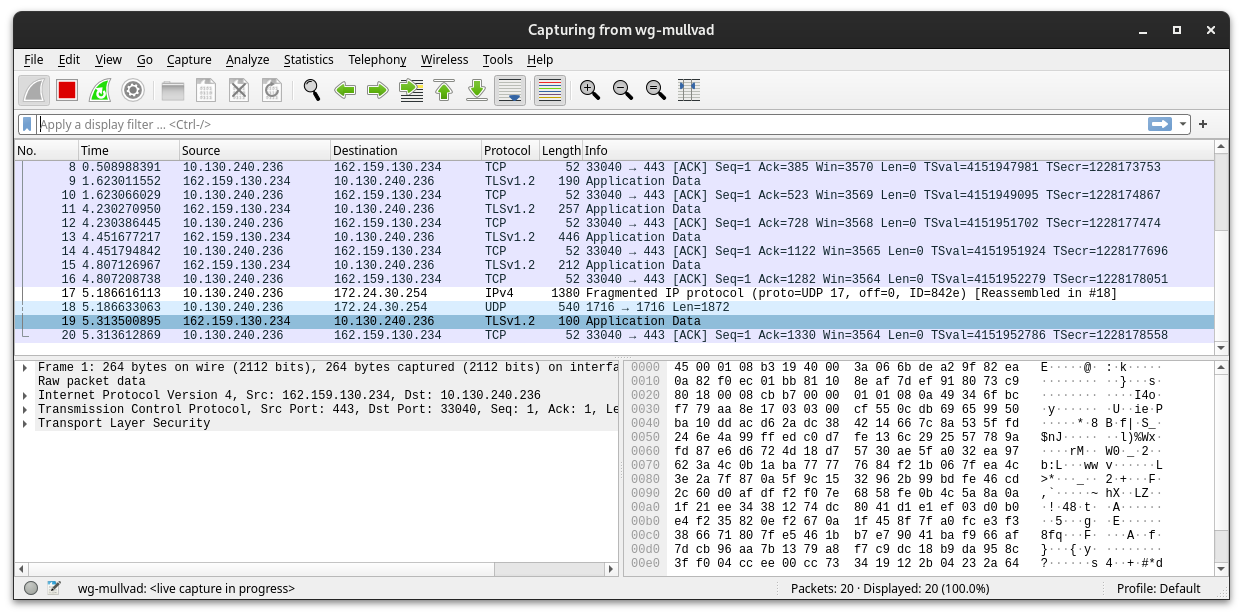
\includegraphics[scale=0.25]{Bilder/Screenshot_1.png}
		\label{fig:figure2}
		\caption{Beispielscreenshot aus der Wireshark Software}
	\end{center}
\end{figure}


\subsection{Funktionsumfang}

Wireshark ist eine Software mit sehr vielen Funktionen. Sie bietet wirklich alles rund um das Thema Netzwerkanalyse. Die wichtigsten Funktionen sind:
\begin{itemize}
	\item Die Verfügbarkeit aus sehr vielen Platformen
	\item Die Möglichkeit dumps von anderen Personen importieren zu können
	\item Das Filtern von Paketen nach sehr vielen Kriterien
\end{itemize}
Besonders die letztere Funktion ist sehr wichtig, da man ohne diese schnell die Orientierung in der Software verlieren kann. \cite{features}

\subsection{Anwendungsbereiche}
Wie im oberen Teil schon dargestellt, hat Wireshark sehr viele Funktionen. Allein deswegen wird es auch als Schweizer Taschenmesser der Netzwerktechnik bezeichnet. Somit kann Wireshark in sehr vielen Situationen Anwendung finden. Es kann beispielsweise von Netzwerk Administratoren benutzt werden, um Netzwerk Probleme  zu Analysieren und zu lösen. Es kann außerdem von Netzwerk Sicherheits Analysten benuzt werden, um Sicherheitsprobleme in Netzwerken zu finden. Wiederum kann es auch von Anwendungsentwicklern benutzt werden, um Netzwerkprotokoll Implementationen zu debuggen. Zuletzt kann es auch benutzt werden um mehr über Netzwerktraffic zu lernen und diesen zu Analysieren. Es gibt natürlich auch viele weitere Möglichkeiten WIreshark zu benutzen. \cite{intendedpurposes}




\newpage



\section{Netzwerk}

\subsection{Aufbau}
\subsection{Protokolle}
% tcp, udp, http(s), tls/ssl,  
% tor

\subsection{Open System Interconnection Modell}


	% Please add the following required packages to your document preamble:
	% \usepackage{multirow}
\begin{wrapfigure}{r}{0pt}
	\centering
	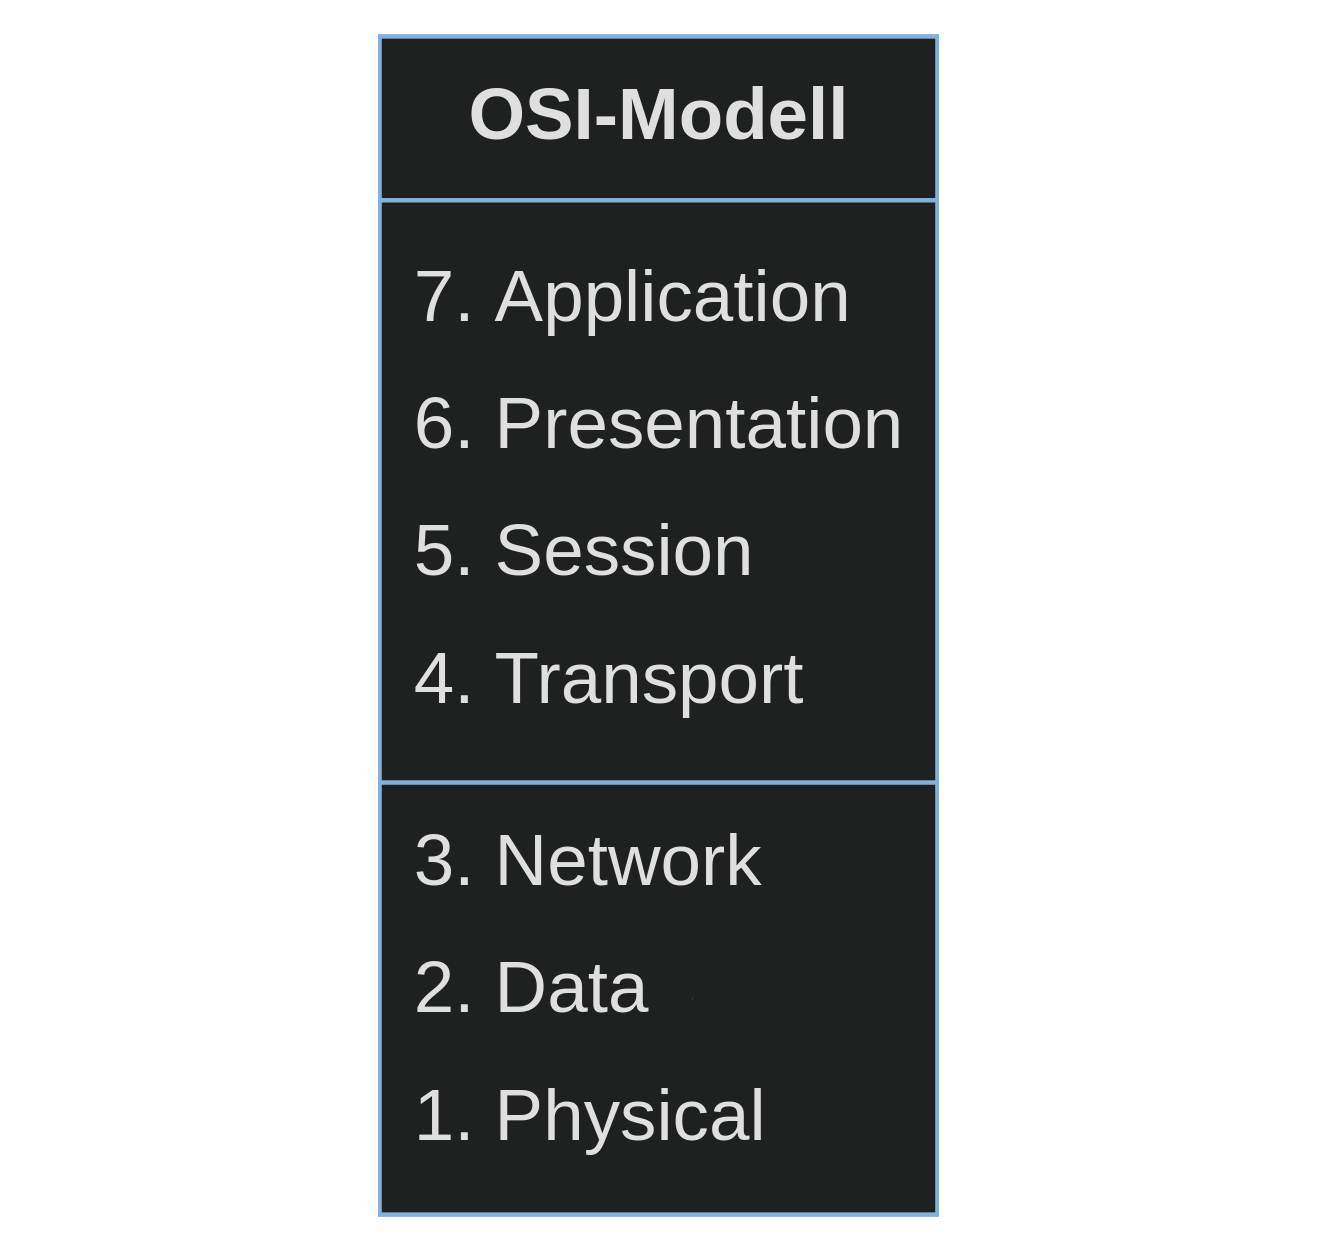
\includegraphics[scale=0.1]{Bilder/OSI-Modell}
	\caption{OSI-Modell}
	\label{fig:figure3}
	
\end{wrapfigure}



	Das Open System Interconnect\footnote{dt: Offenes System für Kommunikationsverbindungen} Modell, auch OSI-Modell genannt, beschreibt die Voraussetzungen, die für eine Kommunikation innerhalb eines Netzwerks nötig sind. Dieses wurde 1983 von durch die `Internationale Organisation für Normung`, kurz `ISO` standardisiert. Dies ist notwendig, damit sich alle Komponenten im Netwerk, auch wenn diese von verschiedenen Herstellern produziert wurden, reibungslos miteinander funktionieren. Wenn ein Paket beispielsweise von einem Computer im Netwerk losgeschickt wird, muss es mehrere Stationen durchlaufen. Das Paket verlässt den Rechner über die Netzwerkkarte und wird durch ein Übertragungsmedium über weitere Netzwerkkomponenten, wie Hubs oder Router bis zur Netzwerkkarte des Zielrechners geleitet. Dort wird dieses dann Interpretiert, um korrekt dargestellt zu werden. All diese Schritte werden durch ein Protokoll festgehalten und durch das OSI-Modell spezifiziert, damit jede Station auf diesem Weg weiß, wohin das Paket möchte, woher es kommt und welche Eigenschaften es hat. So wird ein Standart geschaffen, mit dem alle Computersysteme miteinander kommunizieren können.
	
	Da diese  Datenkommunikation relativ komplex ist, wurde das Modell in sieben Schichten eingeteilt. Die oberen 4 Schichten gehören zu den `Host Layer(n)`\footnote{dt: Anwendungsorientierte Schichten}. Die unteren 3 Schichten werden `Media Layer`\footnote{dt: Transport Schichten} genannt. Jede Schicht behandelt eine Anforderung, die für eine funktionierende Kommunikation erfüllt werden muss. Ein zu übertragenes Paket durchläuft vor der Versendung die Schichten 7 - 2, wobei dem Paket bei jeder Schicht Protokoll-Informationen hinzugefügt werden, die dann im Protokoll des Datenpaketes auffindbar sind. Die erste und letzte Schicht wandelt das Paket in technisch übertragbare Daten um und schickt dieses über das Übertragsmedium weg. Das Übertragsmedium kann hierbei ein Kabel sein, oder aus einer Antenne bestehen. Auf der Empfängerseite wird dieser Prozess rückwärts durchgeführt. Hierbei wird die jeweilige Protokoll-Information nach der Interpretierung durch die jeweilige Schicht entfernt, bis zum Inhalt des Paketes.
	
	Im folgenden werden die einzelnen Schichten  einzeln beleuchtet, um einen besseren Einblick zu gewähren.


\subsubsection{Anwendungsschicht}
	Die Anwendungsschicht\footnote{engl. application layer} stellt die Daten dar, mit welchen der Nutzer interagiert. Softwareanwendungen, wie Web-Browser und E-Mail clients stützen sich auf die siebte Schicht, um dem Nutzer aussagekräftige Daten zu präsentieren. 
	
	Hierzu gehören Protokolle, wie HTTP\footnote{Hyper Text Transfer Protocol}, welches benutzt wird, um Websites welche in HTML\footnote{Hyper Text Markup Language} geschrieben sind zu präsentieren, oder SMTP\footnote{Simple Mail Transfer Protocol}, welches benutzt wird um E-Mails zu präsentieren.

\subsubsection{Präsentationsschicht}
	Die Präsentationsschicht\footnote{engl: presentation layer} ist in erster Linie dafür verantwortlich, die Daten so aufzubereiten, dass diese in der Anwendungsschicht verwendet werden können. Ein wichtiger Teil dabei ist die Verschlüsselung. Die Präsentationsschicht muss, wenn die Geräte durch eine verschlüsselte Verbindung kommunizieren, auf Senderseite eine Verschlüsselung hinzufügen und diese auf der Empfängerseite korrekt dekodieren. 
	
	Ebenso ist die Präsentationsschicht für die Komprimierung der Daten verantwortlich. Dadurch kann die Geschwindigkeit und Effizienz der Kommunikation erhöht und die benötigte Bandbreite minimiert werden.

\subsubsection{Sitzungsschicht}
	Anschließend folgt die Sitzungsschicht\footnote{engl: session layer}. Diese ist für das Öffnen und Schließen der Kommunikation der beiden Geräte zuständig. Hier wird die Kommunikation in Sitzungen eingeteilt. Eine Sitzung reicht von der Öffnung bis zur Schließung der Verbindung. Somit wird sicher gestellt, dass die Sitzung lange genug geöffnet bleibt, um alle Daten zu übertragen. Wenn alle Daten erfolgreich übertragen wurden, leitet die Sitzungsschicht die umgehende Schließung der Sitzung ein, um Ressourcen zu sparen. 
	
	Eine weitere sehr wichtige Aufgabe der Sitzungsschicht ist die Sicherung der Datenverbindung durch synchronisierte Checkpoints. Wenn beispielsweise bei der Übertragung einer 450 Megabyte großen Datei bei 230 Megabyte die Verbindung unterbrochen wird, kann nach einer Neuverbindung die Übertragung bei 230 Megabyte wieder aufgenommen werden, da es einLayer 4 ist für die End-to-End-Kommunikation zwischen den beiden Geräten verantwortlich. Dazu gehört auch, Daten vom Session Layer zu nehmen und sie in Abschnitte zu zerlegen, die Segmente genannt werden, bevor sie an den Layer 3 gesendet werden. Der Transport Layer des Empfangsgeräts ist für die Wiederzusammenstellung der Segmente zu Daten verantwortlich, die der Session Layer verarbeiten kann.
	
	Die Transportebene ist zudem für die Fluss- und Fehlersteuerung zuständig. Die Flusssteuerung bestimmt eine optimale Übertragungsgeschwindigkeit, um sicher zu stellen,  dass ein Sender mit einer schnellen Verbindung einen Empfänger mit einer langsamen Verbindung nicht überfordert. Die Transportebene führt eine Fehlerkontrolle auf der Empfängerseite durch, indem sie sicherstellt, dass die empfangenen Daten vollständig sind, und eine erneute Übertragung anfordert, falls dies nicht der Fall ist.
	
	Zu den Protokollen der Transportschicht gehören Checkpoint der Datei bei 230 Megabyte gibt. Ohne diese Checkpoints müsste der Transfer der Datei von vorne beginnen.

\subsubsection{Transportschicht}
 In der Transportschicht\footnote{engl: transport layer} werden die Datenpakete vor dem Versenden in Segmente zerlegt. Im Empfangsgerät werden die diese Segmente durch die Transportschicht wieder korrekt zusammengesetzt, sodass diese von der Sitzungsschicht benutzt werden können. 
 
 Die Transportebene ist ebenfalls für die Fluss- und Fehlersteuerung zuständig. Hierbei wird die Übertragungsgeschwindigkeit so festgelegt, dass ein ggf. langsamer Empfänger nicht durch die ggf. schnelle Geschwindigkeit des Senders überfordert wird. Beim Empfänger wird durch die Fehlersteuerung ein vollständiger Empfang aller Daten sichergestellt. Wenn die empfangenen Daten nicht vollständig sind, werden diese durch dieses System erneut angefordert, um die Vollständigkeit der Daten zu garantieren. 
 
 Hierzu gehören die Protokolle `Transmission Control Protocol` (TCP) und `User Datagram Protocol` (UDP)
 
 
\paragraph{Exkurs: UDP/TCP}
   
\subsubsection{Bitübertragungsschicht}
\subsubsection{Sicherungsschicht}
\subsubsection{Netzwerkschicht}





\section{Analyse}
\subsection{Beispiel}
\subsection{Browser}
\subsubsection{Mozilla Firefox}
\subsubsection{Microsoft Edge}
 \subsubsection{Mullvad Browser}
\subsubsection{Opera Browser}




 \section{Fazit}

% end of text

\newpage
 \listoffigures
\newpage
\bibliographystyle{plain}
\bibliography{gg}

\newpage

\centering
\vspace*{200pt}
\Huge{\section{Anlagen}}

\end{document}

